\section{$\mathcal{CE}$ Machine} \label{sec:mach}

Using the calculus of cactus environment defined in the previous section, we
derive an abstract machine: the $\mathcal{CE}$ machine\footnote{No relation to
Felleisen and Friedman's CEK machine~\cite{felleisen1986control}}. The syntax
and semantics are defined in Figure~\ref{fig:CEM}. 

\begin{figure*}
\textbf{Syntax}
\begin{align*}
\tag{State} s &::= \langle c, \sigma, \mu, f \rangle \\
\tag{Term} t &::= i \; | \; \lambda t \; | \; t \; t  \\
\tag{Variable} i &\in \mathbb{N}  \\
\tag{Closure} c &::= t [l] \\
\tag{Value} v &::= \lambda t[l] \\
\tag{Heap} \mu &::= \epsilon \; | \; \mu [ l \mapsto \rho ] \\
\tag{Environment} \rho &::= \bullet \; | \; c \cdot l \\
\tag{Context} \sigma &::= \square \; | \; \sigma \; c \;  | \; u:=\sigma \\
\tag{Location} l,u,f &\in \mathbb{N}
\end{align*}
\textbf{Semantics}
\begin{align*}
\tag{Upd}
\langle v, u := \sigma, \mu[u \mapsto c \cdot l], f \rangle 
  &\rightarrow_{\mathcal{CE}}
\langle v, \sigma, \mu[u \mapsto v \cdot l], f \rangle  \\
\tag{Lam}
\langle \lambda t[l], \sigma \; c, \mu, f \rangle 
  &\rightarrow_{\mathcal{CE}}
\langle t[f], \sigma, \mu[f \mapsto c \cdot l], f+1 \rangle  \\
\tag{App}
\langle t \; t'[l], \sigma, \mu, f \rangle
  &\rightarrow_{\mathcal{CE}}
\langle t[l], \sigma \; t'[l], \mu, f \rangle \\
\tag{Var1}
\langle 0[l], \sigma, \mu, f \rangle
  &\rightarrow_{\mathcal{CE}}
\langle c, l := \sigma, \mu, f \rangle 
\; \textnormal{where} \; c \cdot l' = \mu(l)\\
\tag{Var2}
\langle i[l], \sigma, \mu, f \rangle
  &\rightarrow_{\mathcal{CE}}
\langle (i-1)[l'], \sigma, \mu, f \rangle
\; \textnormal{where} \; c \cdot l' = \mu(l)
\end{align*}
\caption{Syntax and semantics of the $\mathcal{CE}$ machine.}
\label{fig:CEM}
\end{figure*}

The machine operates on a similar syntax as the calculus, extended only with a
context to implement the updates from the NVar subderivation ($u:=\sigma$) and
the operands from the NEval subderivation ($\sigma \; c$). We also add $f$
explicitly, which is our fresh heap location. Thus, we now have a 4-tuple, with
initial state $\langle t[0], \square, \epsilon[0=\bullet], 1\rangle$. The four
parts of the tuple are the current closure, the context, the heap, and the fresh
heap location. On the update rule, our current closure is a value, and there is
an update marker as the outermost context. This implies that a variable was
entered, and our current closure represents the corresponding value for that
variable.  Thus, we update the location $u$ that the variable entered, replacing
whatever term was entered with the current closure. The Lam rule takes an
argument off the context and binds it to a variable, allocating a fresh heap
location for the bound variable. This ensures that every instance of the
variable will point to this location, and thus the bound term will only be
evaluated at most once. The App rule simply pushes an argument term in the
current environment. The Var1 rule enters the closure pointed to by the
environment location, while the Var2 rule traverses the cactus environment to
locate the correct closure. The correspondence with the calculus semantics from
the previous section is as follows: The NVar rule is implemented with Var and
Update, and the NEval rule is implemented with Lam and App. 

To get some intuition for the $\mathcal{CE}$ machine and how it works, consider
the depiction in Figure~\ref{fig:state} of its state during evaluation of the
term: $(\lambda a.(\lambda b.b \; a) (\lambda c.c \; a)) ((\lambda i.i) (\lambda
j.j))$. We leave the variable names for readability. For thoroughness, the
occurrences of variable $a$ may be replaced with index $1$, and the rest can be
replaced with index $0$. At this point in the computation, the closure for $a$
is shared, and has been updated with its value. The closure in the context (the
$a$ from the application $c \; a$) now points to the updated value.

\begin{figure}
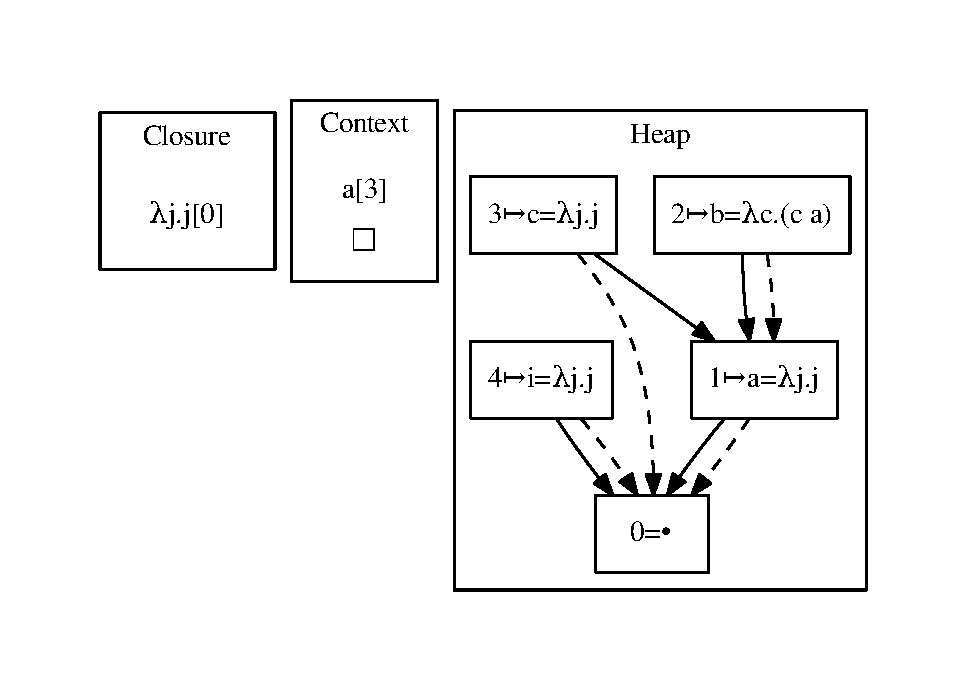
\includegraphics[width=\linewidth]{figures/18.pdf}
The dotted lines represent the environment for the bound closure, and the solid
lines represent the next environment cell:  $t[dotted] \cdot solid$. The
variables are left in for readability, but can be trivially replaced with
deBruijn indices. See Figure~\ref{fig:states} in the Appendix for a
visualization of a number of subsequent machine states. The free Heap location
$f$ is left out to save space.
\caption{$\mathcal{CE}$ machine state example}
\label{fig:state}
\end{figure}

